
\begin{frame}
  \frametitle{PySpice :  The Bridge between SPICE and Python}
  \textbf{How it is born ?}
  \begin{itemize}
  \item Come back to electronic learning
  \item Use the most maintained SPICE flavour : \textbf{NgSpice}
  \item But analysis tools are outdated : e.g. TCL Spice
  \item \textbf{I want Python !!!}
  \end{itemize}
  \vspace{1.5em}
  \centerline{\alert{$\Longrightarrow$ Plug NgSpice to Python}}
  \vspace{1.5em}
  \textbf{How to get it ?}
  \begin{itemize}
  \item \url{https://pyspice.fabrice-salvaire.fr}
  \item \url{https://github.com/FabriceSalvaire/PySpice}
  \item Available on PyPi
  \item Licensed under GPLv3
  \end{itemize}
\end{frame}

\begin{frame}
  \frametitle{PySpice: Workflow}
  \begin{center}
    \begin{tikzpicture}%
      [node distance=10mm,
      start chain=going right,
      >=stealth',
      punktchain/.style={
        rectangle,
        rounded corners,
        % fill=black!10,
        draw=black, very thick,
        text width=7em,
        minimum height=2em,
        text centered,
        on chain},
      line/.style={draw, thick, <-},
      every join/.style={->, thick,shorten >=1pt},
      ]
      \node[punktchain, join] {Python Netlist};
      \node[punktchain, join] {NgSpice};
      \node[punktchain, join] {Python Analysis};
    \end{tikzpicture}
  \end{center}
  \vspace{.5em}
  \begin{columns}[T]
    \begin{column}{.55\textwidth}
      \begin{enumerate}
      \item Define circuit in Python \\
        {
          \footnotesize
          \text{\colorR{C}\colorM{in} \colorB{1 2} \colorG{470n}}
          $\longrightarrow$
          \text{circuit.\colorR{C}(\colorM{'in'}, \colorB{1, 2}, \colorG{nano(470)})} \\[.5em]
        }
        or include netlist as is
      \item Define simulation parameters \\
      \item Generate netlist code \\
      \item Execute NgSpice {\tiny (server mode)} \\
      \item Get output as Numpy array
      \item Analyse, plot \ldots
      \end{enumerate}
    \end{column}
    \begin{column}{.45\textwidth}
      Why Python Netlist ?
      \begin{itemize}
      \item More verbose, \textbf{But}
      \item Can use Python to configure netlist
        \href{https://pyspice.fabrice-salvaire.fr/examples/diode/voltage-multiplier.html}{example}
      \item keyword argument \\
        \texttt{resistance=kilo(100)} \\[.5em]
      \item cf. Modelica \tiny{see later}
      \end{itemize}
    \end{column}
  \end{columns}
\end{frame}

\begin{frame}
  \frametitle{PySpice: I hate Netlist, I want a Schematic Editor !!! }
  \centerline{\textbf{No Problem, Use \href{http://kicad-pcb.org}{KiCad}!}}
  \vspace{1em}
  \begin{columns}
    \begin{column}{.6\textwidth}
      \begin{itemize}
      \item Implement a minimal Netlist parser
      \item \alert{But a full parser would be difficult to implement} \\
        NgSpice syntax is very complex \\
        due to many extensions \\
        % And any grammar
      \item Tips: Use subcircuit to hide complexity
      \end{itemize}
    \end{column}
    \begin{column}{.4\textwidth}
      \begin{center}
        Leading Open Source \\
        Electronics Design Automation Suite \\[1em]
        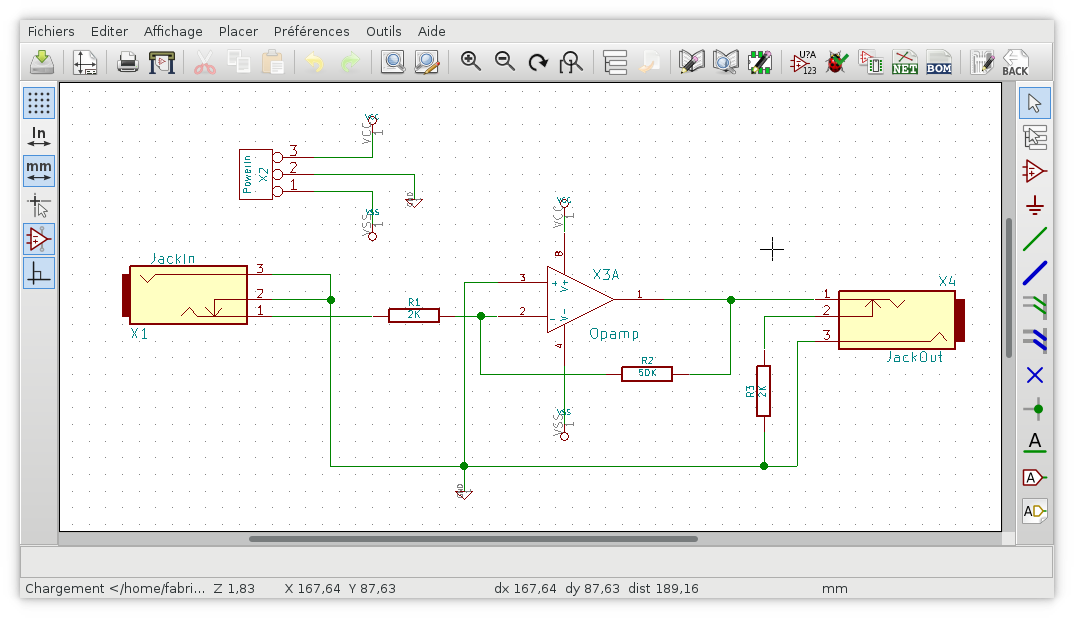
\includegraphics[width=1.\textwidth]{images/kicad.png}
      \end{center}
    \end{column}
  \end{columns}
  \vspace{1em}
  \centerline{\small \href{https://pyspice.fabrice-salvaire.fr/examples/spice-parser/kicad-example.html}{KiCad example}}
\end{frame}

\begin{frame}
  \frametitle{PySpice: NgSpice as a Shared Library}
  \begin{itemize}
  \item NgSpice can be used as a shared library instead of an executable
  \item Not a big improvement, \textbf{But}
  \item We can use the \textbf{NgSpice Shared API}
    \begin{itemize}
    \item To define external independent voltage/current sources (Input) % \\
      % API defines callback \\
      % \texttt{int (GetVSRCData)(double*, double, char*, int, void*)} \\
      % \texttt{int (GetISRCData)(double*, double, char*, int, void*)}
    \item To get the simulation output at each step (Output)
    \end{itemize}
    \begin{center}
      \begin{tikzpicture}
        [node distance=20mm,
        start chain=going right,
        >=stealth',
        punktchain/.style={
          rectangle,
          rounded corners,
          % fill=black!10,
          draw=black, very thick,
          text width=6em,
          minimum height=3em,
          text centered,
          on chain},
        line/.style={draw, thick},
        ]
        \node[punktchain] (p) {Python / C};
        \node[punktchain] (n) {NgSpice};
        \draw[->, thick] ($ (p.east) + (0,.5em) $) -- node[above] {sources} ($ (n.west) + (0,.5em) $);
        \draw[<-, thick] ($ (p.east) - (0,.5em) $) -- node[below] {output} ($ (n.west) - (0,.5em) $);
      \end{tikzpicture} \\
      \alert{We can thus extend NgSpice easily with C or Python code}
    \end{center}
  \item API also features a step by step simulation mode
  \item PySpice as a \href{http://cffi.readthedocs.io/en/latest/}{CFFI} Binding
  \end{itemize}
  \vspace{1em}
  \centerline{\small \href{https://pyspice.fabrice-salvaire.fr/examples/ngspice-shared/voltage-divider.html}{NgSpice API example}}
\end{frame}

\begin{frame}[fragile]
  \frametitle{PySpice: Example's Documentation Generator}
  \centerline{\textbf{PySpice has some learning materials}}
  \begin{columns}[T]
    \begin{column}{.6\textwidth}
      \begin{itemize}
      \item Kind of Jupyter Notebook \ldots \\
        but for peoples who want a \textbf{True Editor} \\
        {\small Emacs} {\tiny or vi if you like}
      \item \href{http://docutils.sourceforge.net/rst.html}{reStrucuredText} and \href{http://www.sphinx-doc.org}{Sphinx}
      \item \href{https://ece.uwaterloo.ca/~aplevich/Circuit_macros/}{Circuit\_macros} for diagrams % {\tiny with M4 macros inside !}
      \item Concept: Use directive comments \\
        to add text and figure blocks
      \end{itemize}
    \end{column}
    \begin{column}{.4\textwidth}
      \fontsize{4.5pt}{4.5pt}\selectfont
\begin{Verbatim}[commandchars=\\\{\}]
\colorO{# A source code comment}
\colorR{#?# A comment that must not appear in the documentation}

\colorB{#!# ==========================}
\colorB{#!#  A Restructuredtext Title}
\colorB{#!# ==========================}

python code ...

\colorB{#!#}
\colorB{#!# Some reStructuredText contents}
\colorB{#!#}

python code ...

\colorO{# Insert the output of the following python code}
python code ...
\colorM{#o#}

\colorO{# Add the file content as literal block}
\colorM{#itxt# kicad-pyspice-example/kicad-pyspice-example.cir}

\colorO{# Add a Python file as a literal block}
\colorM{#i# RingModulator.py}

\colorO{# Insert an image}
\colorM{#lfig# kicad-pyspice-example/kicad-pyspice-example.sch.svg}

\colorO{# Insert Circuit_macros diagram}
\colorM{#cm# circuit.m4}

\colorO{# Insert a Matplotlib figure}
\colorM{#fig# save_figure(figure, 'my-figure.png')}
\end{Verbatim}
      \normalsize
    \end{column}
  \end{columns}
\end{frame}

\begin{frame}[fragile]
  \frametitle{Diagrams with Circuit\_macros \ldots or Algorithms versus GUI}
  \begin{columns}
    \begin{column}{.5\textwidth}
      \fontsize{6pt}{6pt}\selectfont
\begin{Verbatim}[commandchars=\\\{\}]
.PS
cct_init

elen = 0.75
epsilon = 1e-3

G: \colorR{ground}; \colorB{dot}; "0" \colorB{rjust}
  \colorR{source}(\colorO{up_} elen, AC); \colorB{llabel}(,V_{in},); \colorB{dot}; "in" \colorB{rjust}
  \colorR{capacitor}(\colorO{right_} elen); \colorB{llabel}(,C_{1},); \colorB{dot}; "2" \colorB{rjust above}
  \{ \colorR{resistor}(\colorO{down_} \colorO{to} (Here,G)); \colorB{rlabel}(,R_{2}) \}
  \{ R1: \colorR{resistor}(\colorO{up_} elen_*1.5); \colorB{llabel}(,R_{1}); \colorB{dot}; "5" \colorB{above} \}

  line \colorO{right_} elen_/2; \colorO{up_}
Q1: \colorR{bi_tr}(,,,E) \colorO{with} .B \colorO{at} \colorO{Here}; \colorB{llabel}(,,Q_1)

Q1E: Q1.E - (0,elen_/8)
  \colorB{line} \colorO{down} \colorO{from} Q1.E \colorO{to} Q1E; \colorB{dot}; "3" \colorB{ljust}
  \colorR{resistor}(\colorO{down_} \colorO{to} (Q1.E,G)); \colorB{rlabel}(,R_{E})

Q1C: Q1.C + (0,elen_/8)
  \colorB{dot}(\colorO{at} Q1C); "4" \colorB{ljust above}
  \colorR{capacitor}(\colorO{right_} elen \colorO{from} Q1C); \colorB{llabel}(,C_{2})
  \colorB{dot}; "out" \colorB{ljust}
  \colorR{resistor}(\colorO{down_} \colorO{to} (Here,G)); \colorB{rlabel}(,R_{L})
  \colorB{line} \colorO{down} epsilon \colorO{then} \colorO{to} G

  \colorR{resistor}(\colorO{up_} \colorO{from} Q1.C \colorO{to} (Q1.C,R1.end)); \colorB{llabel}(,R_{C})
  \colorB{line} \colorO{up} epsilon \colorO{then} \colorO{left} \colorO{to} (G,R1.end) \colorO{then} \colorO{down} epsilon
  \colorR{reversed}(`source', \colorO{down_} elen, V); \colorB{llabel}(,V_{pwr},)
  \colorR{ground}
.PE
\end{Verbatim}
      \normalsize
      {\tiny Also \href{http://www.texample.net/tikz/examples/tag/circuitikz}{circuitikz}}
    \end{column}
    \begin{column}{.5\textwidth}
      \begin{center}
        \textbf{With M4 macros inside !} \\
        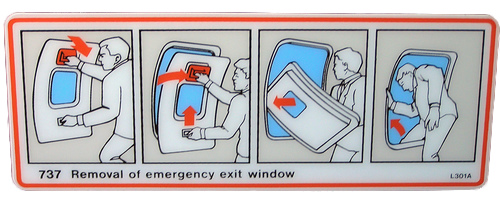
\includegraphics[width=.6\textwidth]{images/emergency-exit-1.jpg} \\ %[.5em]
        m4 $\rightarrow$ dpic $\rightarrow$ \href{http://www.texample.net/tikz}{tikz} $\rightarrow$ \LaTeX \\
        \includegraphics[width=.6\textwidth]{figures/ac-coupled-amplifier.pdf}
      \end{center}
    \end{column}
  \end{columns}
\end{frame}

%%% Local Variables:
%%% mode: latex
%%% TeX-master: "master"
%%% End:
